%!TEX spellcheck
%!TEX root = ../bachelor_paper.tex
\documentclass[../bachelor_paper.tex]{subfiles}
\graphicspath{{\subfix{images/}}}
\begin{document}

\chapter{Hardware impact}
    \label{ch:perf}
    
We have observed an expected increase in resource utilization on the \ac{SoC}. Datalynx requires additional \acp{LUT}, \acsp{LUTRAM}, \acp{FF}, as well as one additional \ac{BUFG} as seem in Table \ref{tab:perf/util/data}. According to the timing analysis performed by Vivado, our worst slack stayed about the same slightly improving from 1.316ns to 1.767ns with the total negative slack being 0ns. Hold slack also slightly improved from 0.054ns to 0.055ns with total negative hold slack again being 0ns. As we have not changed the implementation of the core itself, the additions should be completely transparent to a workload run on the processor, as long as the core frequencies are unchanged. While the critical path for setup slack has not changed in the modified design, the path for hold slack actually has, as can be seen in table \ref{tab:perf/timing/crit}. However, this occurs within the block diagram wrapper generated by Vivado and does not worsen overall hold slack performance significantly. Additionally, this change is likely caused by high utilization of the chip overall and the resulting less than ideal routing results. We thus see this change in critical path as a minor issue albeit something to be aware of.

Of note is the increase in power draw according to Vivado. This metric is far from accurate, as these power metrics are dependent on Vivado's randomized optimizations, meaning different runs will yield sightly different reported power characteristics. Additionally, due to the nature of this implementation, higher power draw is expected as two additional cores have been enabled on the chip. A different implementation might choose a more minimalist method for offloading data from the chip, significantly lowering power draw impact.\\
In our synthesis run, Vivado estimated about 0.391W power draw for the unmodified and 1.996W power draw for the modified design. \\
As seen in Figure \ref{fig:perf/power/split}, the share of dynamic power losses increases significantly with the inclusion of the \ac{PS7}. This block alone makes up about 81\% of power drawn in the modified system. When excluded, power consumption only rises by 76mW compared to the original design. This is still a skewed value however, as other \acp{IP} by Xilinx, like the GPIOs and AXI crossbar unit have not been excluded. Including the \ac{PS7} for the modified design leaves us with an estimated junction temperature of roughly 48.0\textdegree C for the modified and 29.5\textdegree C for the unmodified design, resulting in a 37.0\textdegree C and 55.5\textdegree C temperature margin respectively.

\begin{table}
    \centering
    \resizebox{\textwidth}{!}{%
    \begin{tabular}{lll}
    \textbf{Design} & \textbf{Path} \\
    \hline\\[-0.9em]
    \textbf{Unmodified} & From  & \texttt{i\_pulpissimo/soc\_domain\_i/pulp\_soc\_i/jtag\_tap\_top\_i/tap\_top\_i/ td\_o\_reg/C} \\
                        & To    & \texttt{pad\_jtag\_tdo} \\
                        & Setup & 1.32ns \\
    \textbf{Modified}   & From  & \texttt{i\_pulpissimo/soc\_domain\_i/pulp\_soc\_i/jtag\_tap\_top\_i/tap\_top\_i/ td\_o\_reg/C} \\ 
                        & To    & \texttt{pad\_jtag\_tdo} \\
                        & Setup & 1.77ns \\
    \textbf{Unmodified} & From  & \texttt{i\_pulpissimo/soc\_domain\_i/pulp\_soc\_i/soc\_peripherals\_i/i\_apb\_adv\_timer/u\_apb\_if/r\_timer1\_th\_reg[9]/C} \\
                        & To    & \texttt{i\_pulpissimo/soc\_domain\_i/pulp\_soc\_i/soc\_peripherals\_i/i\_apb\_adv\_timer/u\_tim1/u\_counter/r\_start\_reg[9]/D} \\
                        & Hold  & 0.05ns \\
    \textbf{Modified}   & From  & \texttt{datalynx\_wrapper\_i/datalynx\_i/axi\_gpio\_4/U0/ip2bus\_data\_i\_D1\_reg[11]/C} \\
                        & To    & \texttt{datalynx\_wrapper\_i/datalynx\_i/axi\_gpio\_4/U0/AXI\_LITE\_IPIF\_I/ I\_SLAVE\_ATTACHMENT/s\_axi\_rdata\_i\_reg[20]/D} \\
                        & Hold  & 0.05ns \\
    \hline
    \end{tabular}}
    \caption{Critical paths for setup and hold slack in unmodified and modified design}
    \label{tab:perf/timing/crit}
\end{table}
\begin{table}
    \centering
    \resizebox{\textwidth}{!}   & \textbf{Utilization}  & \textbf{Utilization \%}   & \textbf{Change}   \\
                        &                       & \textbf{unmodified}   & \textbf{unmodified}       & \textbf{modified}     & \textbf{modified}         &                   \\
    \hline
    \acs{LUT}           & 53200                 & 43502                     & 81.77\%                       & 46432                     & 87.28\%   & +6.7\%\\
    \acs{LUTRAM}        & 17400                 & 12                        & 0.07\%                        & 74                        & 0.43\%    & +516.7\%\\
    \acs{FF}            & 106400                & 22526                     & 21.17\%                       & 28214                     & 26.52\%   & +25.3\%\\
    \acs{BRAM}          & 140                   & 128                       & 91.43\%                       & 128                       & 91.43\%   & +0\%\\
    \acs{DSP}           & 220                   & 12                        & 5.45\%                        & 12                        & 5.45\%    & +0\%\\
    \acs{IO}            & 200                   & 38                        & 19.00\%                       & 38                        & 19.00\%   & +0\%\\
    \acs{BUFG}          & 32                    & 9                         & 28.13\%                       & 10                        & 31.25\%   & +11.1\%\\
    \acs{MMCM}          & 4                     & 2                         & 50.00\%                       & 2                         & 50.00\%   & +0\%\\
    \hline
    \end{tabular}}
    \caption{Resource utilization unmodified vs. modified}
    \label{tab:perf/util/data}
\end{table}

\begin{figure}
    \centering
    \begin{subfigure}{0.45\textwidth}
        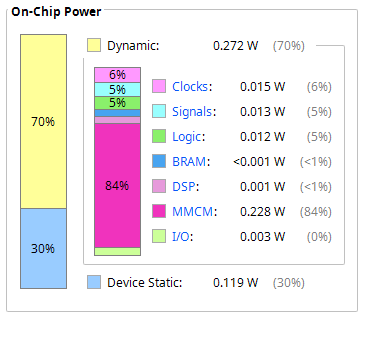
\includegraphics[width=\textwidth]{img/unmodified_power}
        \caption{Unmodified design}
        \label{fig:perf/power/split/unmod}
    \end{subfigure}
    \hfil
    \begin{subfigure}{0.45\textwidth}
        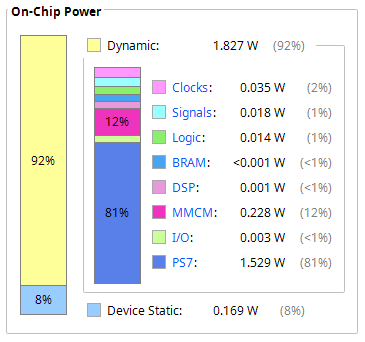
\includegraphics[width=\textwidth]{img/modified_power}
        \subcaption{Modified design}
        \label{fig:perf/power/split/mod}
    \end{subfigure}
    \caption{Estimated power consumption according to Vivado}
    \label{fig:perf/power/split}
\end{figure}

% Render bibliograhy and acronyms if rendered standalone
\isstandalone
\bibliographystyle{IEEEtran}
\bibliography{bibliography}
\subfile{abbreviations.tex}
\fi

\end{document} 
